\documentclass[12pt,a4paper]{article}
\usepackage[utf8]{vietnam}
\usepackage{fontspec}
\setmainfont{Times New Roman}
\usepackage{indentfirst}
\usepackage{hyperref}
\usepackage{tikz}
\usepackage[left=2.64cm,right=2.54cm,top=2cm,bottom=2cm]{geometry}
\usepackage{geometry}
\usepackage{array}
\usepackage{color}
\usepackage{wallpaper}
\setcounter{page}{2}
\makeatletter
\definecolor{dkgreen}{rgb}{0,0.6,0}
\definecolor{gray}{rgb}{0.5,0.5,0.5}
\definecolor{mauve}{rgb}{0.58,0,0.82}
\usepackage{listings}
\pagenumbering{arabic}
\usepackage{fancyhdr}
\usepackage{lastpage}
\usepackage{minitoc}
\pagestyle{fancy}
\fancyhf{}
\rhead{21127511 Nguyễn Quốc Huy}
\lhead{Vật lý đại cương}
\rfoot{Trang \thepage \hspace{1pt}  \pageref{LastPage}}
\usepackage{multicol}
\setlength{\columnsep}{1cm}
\begin{document}
\thispagestyle{empty}
\begin{LARGE}
    \begin{center}{\underline{\color{red}{\bf NATIONAL UNIVERSITY OF HO CHI MINH CITY}}}
    \end{center}
\end{LARGE}
\vspace*{1cm}
\begin{center}{\Huge \color{green}\textbf{KHOA CÔNG NGHỆ THÔNG TIN}}
\end{center}
\ThisCenterWallPaper{1}{New_KHTN.jpg}
\vspace*{15cm}
\begin{center}{\Huge \color{cyan}\textbf{Nguyễn Quốc Huy - 21127511}}
\end{center}
\vspace*{1cm}
\begin{center}
    {\Huge \color{cyan}\textbf{{LỚP 21CLC02 - VẬT LÝ ĐẠI CƯƠNG}}}
\end{center}
\newpage
\let\cleardoublepage\clearpage

\tableofcontents

\newpage
\section{\textbf{\color{red}CHƯƠNG 5 6 : KHÍ LÝ TƯỞNG}}
\Large \subsection{\color{blue}\textbf{BÀI 1} }
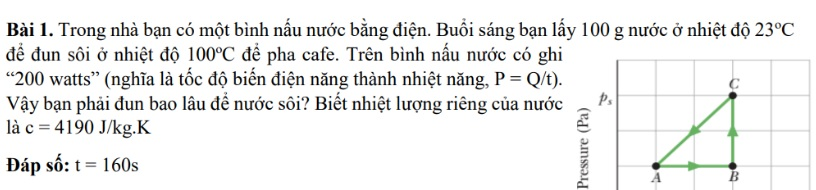
\includegraphics[scale=1]{No.1.jpg}

Ta có $: Q = m.C.\Delta t = 0,1.4190.(100 - 23) = 32263 (J)$

\vspace*{1cm}
$ P = \frac{Q}{t} \Rightarrow t = \frac{Q}{P} = \frac{32263}{200} \approx 161 (s)$
\Large \subsection{\color{blue}\textbf{BÀI 2} }
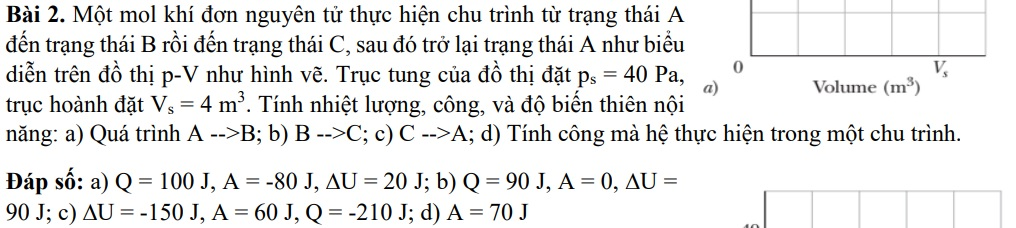
\includegraphics[scale=1]{No.2.jpg}

\vspace*{1cm}
A/ Ta có $Q = \frac{m}{\mu}.C_p.\Delta T = (\frac{i}{2} + 1).\frac{m}{\mu}.R.(T_A - T_B) $

\vspace*{1cm}
$\Leftrightarrow (\frac{i}{2}+1).p.(V_B - V_A)$

\vspace*{1cm}
$\Leftrightarrow (\frac{3}{2}+1).20.(3-1) = 100 (J)$

\vspace*{1cm}
$Vì A \rightarrow B $ là quá trình đẳng áp $ \Leftrightarrow  A = - \int_{V_1}^{V_2} p \,d $

\vspace*{1cm}
$\Leftrightarrow A = - \int_{1}^{3} 20 = - 40 (J) $

\vspace*{1cm}
Độ biến thiên $\Delta U = A + Q = 60 (J)$

\vspace*{1cm}
B/

$Vì B \rightarrow C $ là quá trình đẳng tích $ \Leftrightarrow  A = - \int_{V_1}^{V_2} p \,d = 0$

\vspace*{1cm}
$Q = \frac{i}{2}.(p_C.V_C - p_B.V_B) = \frac{3}{2}.(40.3 - 20.3) = 90 (J)$

\vspace*{1cm}
Độ biến thiên : $\Delta U = A + Q = 90 (J)$

\vspace*{1cm}
C/

\vspace*{1cm}
Độ biến thiên $\Delta U = \frac{i}{2}.(p_A.V_A - p_C.V_C) = \frac{3}{2}.(20.1 - 40.3) = -150 (J)$

\vspace*{1cm}
Từ $C \rightarrow A \Leftrightarrow p = 10V + 10$

\vspace*{1cm}
$\Leftrightarrow$ Công $ A = \int_{V_C}^{V_A} (10V + 10) \,dV = 60 (J)$

\vspace*{1cm}
Nhiệt lượng $Q = A - \Delta U = -150 - 60 = -210 (J)$

\vspace*{1cm}
D/ Công của cả chu trình : 

\vspace*{1cm} 
$A = A_{AB} + A_{BC} + A_{CA} = -40 + 0 + 60 = 20 (J)$

\Large \subsection{\color{blue}\textbf{BÀI 3} }
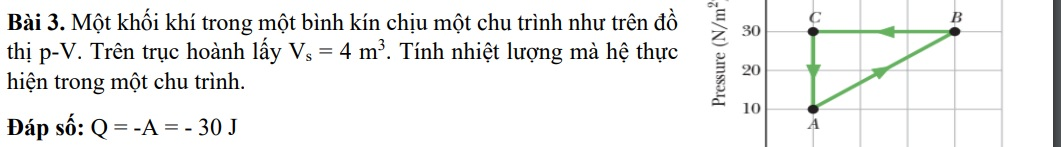
\includegraphics[scale=1]{No.3.jpg}

\vspace*{1cm}
Từ $B \rightarrow C$ : Đẳng áp 

\vspace*{1cm}
$\Leftrightarrow A = -p.(V_C - V_B) = -30.(1-4) = 90 (J)$

\vspace*{1cm}
Từ $C \rightarrow A$ : Đẳng tích $\Leftrightarrow $ Công $A = 0$

\vspace*{1cm}
Từ $A \rightarrow B \Leftrightarrow p = \frac{20}{3}.V + \frac{10}{3}$

\vspace*{1cm}
$\Leftrightarrow $ Công $ A = - \int_{V_A}^{V_B} (\frac{20}{3}V + \frac{10}{3}) \,dV = - \int_{1}^{4} (\frac{20}{3}V + \frac{10}{3}) \,dV  = -60 (J)$

\vspace*{1cm}
$\Leftrightarrow$ Tổng công cả chu trình $A = A_{AB} + A_{BC} + A_{CA} = -60 + 90 + 0 = 30 (J)$

\vspace*{1cm}
Vì là hệ kín $ \Leftrightarrow$ Nhiệt lượng chu trình : $ Q = - A = - 30 (J)$

\end{document}